\documentclass[a4paper,zihao=5,UTF8,fontset=fandol]{phyreport}

\usepackage{caption}
\usepackage{csvsimple}
\usepackage{multicol}
\usepackage{multirow}
\usepackage{booktabs}
\usepackage{siunitx}
\usepackage{subfigure}
\expName{基于Comsol的卡门涡街实验}
\expDate{2023}{10}{}
\subDate{2023}{}{}

\begin{document}
\phyExpCover
\section{实验目的}
学习Comsol模拟仿真软件,用Comsol软件模拟卡门涡街(圆柱绕流)

了解卡门涡街的基础知识,模拟流体经过圆柱后的卡门涡街尾迹

绘制不同时刻的升力系数和曳力系数,分析卡门涡街频率和圆柱体受力

\longLine
\section{实验原理}
\subsection{卡门涡街}
卡门涡街(kormon's vortex street)定常来流绕过某些物体时,在特定条件下会出现不稳定的边界层分离,阻流体下游的两侧会周期性地脱落出旋转方向相反、排列规则的双列线涡,这两排旋涡相互交错排列,就像街道两边的街灯一样。

雷诺数:运动物体上的惯性力与黏性力之比。
$Re = \frac{\rho vL}{\mu}$
雷诺数是用来表征流体流动情况的无量纲数。利用雷诺数可区分流体的流动是层流或湍流,也可用来确定物体在流体中流动所受到的阻力。


卡门涡街形成条件:$47<Re<10^5$

涡振原理(伯努利方程):
\begin{equation}
  \frac{P}{\rho g}+\frac{v^2}{2g}=H  
  \label{eq:bernoulli}
\end{equation}

在流体中安置阻流体,在雷诺数在某一范围内。会出现不稳定的边界层分离,阻流体下游的两侧搓出两道非对称交错排列的旋涡。尾涡脱落的一侧速度增大,压强就减小,尾涡交替脱落,导致圆柱背流面压力交替减小,形成涡振

\subsection{有限元方法}
空间和时间相关问题的物理定律通常用偏微分方程(PDE)描述。对大多数实际问题,这些偏微分方程没有解析解。不过,通常可以把实际模型离散化,用数值的方法进行求解。有限元法(FEM)是工程和数学建模中常用的数值求解偏微分方程的方法,被广泛应用于结构力学、流体力学、热传导和电磁学等领域。有限元法最早是在20世纪40年代被德裔美国数学家Richard Courant首次提出,它的基本思想是把一个大系统细分为更小、更简单的部分,称为有限元。在每个有限元上都可以得到一个简单方程。这样,就把原来的偏微分方程变成一个更大的方程组,这个方程组可以模拟整个问题。最后,FEM通过变分法最小化误差函数得到方程的解。

\subsection{COMSOL}
COMSOL是一个集成了有限元法、求解器和建模工具的仿真软件,可以仿真多物理场耦合,为处理各类工程或物理提供了统一的操作界面和工作流程。

\textbf{COMSOL的工作流程:}\\
1. 几何建模\\
2. 物理场设置\\
3. 网格划分\\
4. 研究和优化\\
5. 求解\\
6. 可视化和结果分析

注意:建模时根据具体问题选择合适的建模方法和求解器。比如本实验研究“流过圆柱体后的卡门涡街”,因为不考虑垂直方向的流动,可以选“流体流动”模块的二维层流,求解器可选通用求解器。

\longLine
\section{实验仪器}
使用COMSOL软件

\longLine
\section{实验内容}

\subsection{模型与参数}
本实验研究流体流经圆柱体后的卡门涡街现象,不考虑沿圆柱体方向的流动,因此可在圆柱体的横切面内进行仿真。建模时选择二维层流,让圆柱位于一个长方形内的左端,流体从左端流入,右端流出(如下图所示)。
\begin{figure}[H]
  \centering
  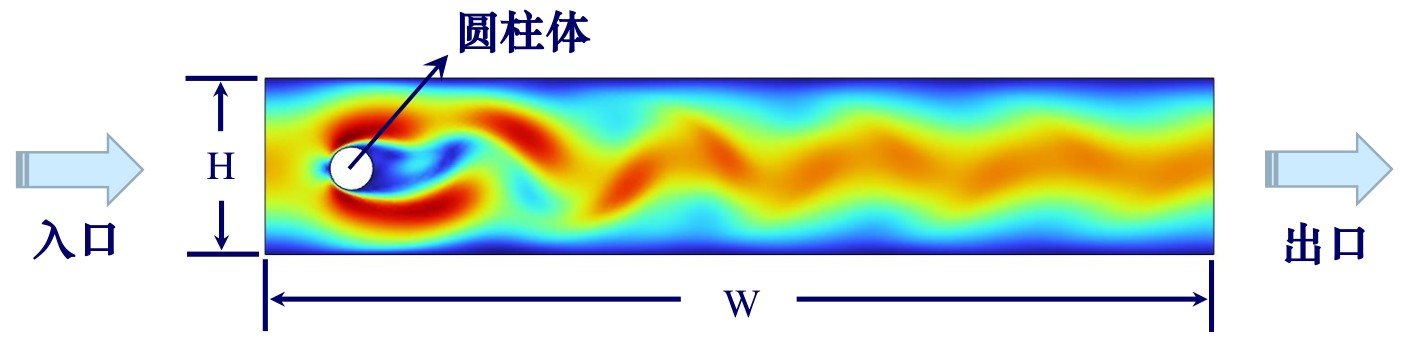
\includegraphics[width=0.8\linewidth]{示意图.png}
  \caption{建模示意图}
\end{figure}
采用的参数值为:流速$u=\qty{1}{m/s}$,流体流过区域的宽度$W=\qty{2.2}{m}$,高度$H=\qty{0.41}{m}$,圆柱半径$R=\qty{0.05}{m}$,圆柱中心与左侧和下边界的距离均为$\qty{0.2}{m}$ 。 流体密度 $\rho= \qty{1}{kg/m^3}$,动力粘度$\mu=\qty{e-3}{Pa\cdot s}$

注:设置中使圆柱体略偏离中心,以触发涡流。

\subsection{纳维-斯托克斯方程、质量守恒方程}
实验中圆柱是固体,流体假设是不可压缩的。需要考虑的耦合为流体-固体耦合,求解的方程是
\begin{equation}
  \rho\frac{\partial \mathbf{u}}{\partial t}+\rho\mathbf{u}\cdot\nabla\mathbf{u}=-\nabla p+\mu\nabla^2\mathbf{u}+\mathbf{f}
\end{equation}
\begin{equation}
  \frac{\partial \rho}{\partial t}+\nabla\cdot(\rho\mathbf{u})=0
\end{equation}
其中$\mathbf{u}$是速度场,$p$是压强场,$\rho$是密度场,$\mu$是动力粘度,$\mathbf{f}$是体积力,这里取为重力加速度$\mathbf{g}$。

这个方程比较复杂,但COMSOL自带的通用求解器可以直接求解。

由于我们更关注流经圆柱体附近的气流,故在入口处设置流体的初速度沿高度方向呈抛物线分布,如右图所示。实验中还使用一个阶跃函数逐渐提升流入速度。
\begin{figure}[H]
  \centering
  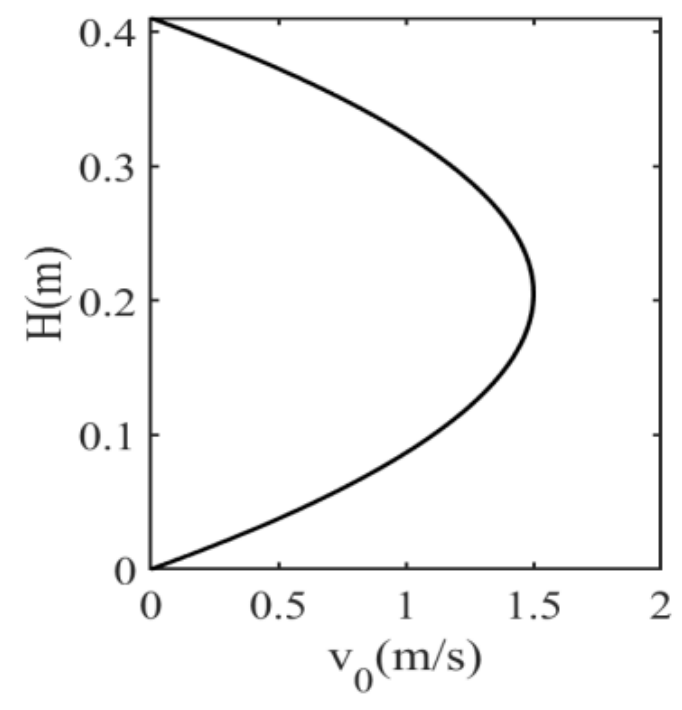
\includegraphics[width = 0.4\linewidth]{抛物线速度分布.png}
  \caption{抛物线速度分布}
\end{figure}
流体的速度随时间在变化,所以求解时选择“瞬态”。圆柱体在流体中的受力可投影为水平方向的曳力($F_D$)和竖直方向的升力($F_L$)。

升力和曳力也随时间变化。因此,相对求解升力和曳力本身,无量纲的升力系数$C_L$和曳力系数$C_D$ :
\begin{equation}
  C_L=\frac{F_L}{\frac{1}{2}\rho u^2R},\quad
  C_D=\frac{F_D}{\frac{1}{2}\rho u^2R}
  \label{eq:CLCD}
\end{equation}

其中$U_{mean}$是设置的平均速度,$\rho$是流体密度, $A$是圆柱在流速方向的投影面积(圆柱厚度与直径的乘积)。

\subsection{实验步骤}
1. 模型向导\\
1.1 打开COMSOL软件,在新建窗口中单击模型向导;\\
1.2 在模型向导窗口中,单击二维;\\
1.3 在选择物理场树中双击流体流动-单向流-层流;\\
1.4 单击添加,然后单击下方的研究;\\
1.5 在选择研究中选择一般研究-瞬态;\\
1.6 单击底部的完成;

2. 参数定义\\
2.1 在左侧模型开发器窗口的全局定义节点下,单击参数1;\\
2.2 在参数的设置窗口中,定位到参数栏;\\
2.3 在表中输入设置\\
2.4 在左侧主屏幕工具栏中单击数,选择全局-阶跃;\\
2.5 在阶跃的设置窗口中,定位到参数栏;\\
2.6 在位置文本框中输入0.1;

3. 几何建模\\
3.1 在上方的几何工具栏中单击矩形;\\
3.2 在矩形的设置窗口中,定位到大小和性质栏;\\
3.3 在宽度文本框输入W,在高度文本框输入H;\\
3.4 单击构建选定对象;\\
3.5 在上方的几何工具栏中单击圆;\\
3.6 在圆的设置窗口中,定位到大小和性质栏;\\
3.7 在位置栏的x文本框输入0.2,在y文本框输入0.2;\\
3.8 定位到大小和形状栏,在半径文本框中输入R;\\
3.9 单击构建选定对象。\\
3.10 在上方的几何工具栏中单击布尔操作和分割,然后选择差集;\\
3.11 在差集的要添加的对象框里添加r1(点击右侧矩形即可添加);\\
3.12 在差集的要减去的对象下方激活选择(点击激活选择按钮即可)\\
3.13 在差集的要减去的对象框里添加c1(点击右侧的圆即可添加);\\
3.14 在几何工具栏中单击全部构建;

4. 材料设置\\
4.1 在模型开发器窗口的组件(comp1)节点下,右键单击材料并选择空材料;\\
4.2 在材料的设置窗口中,定位到材料属性明细栏;\\
4.3 在表中输入设置

5. 层流设置\\
5.1 在模型开发器窗口的组件1(comp1)节点下,右键单击层流(spf)并选择入口;\\
5.2 在入口的设置窗口中,边界选择栏里选择边界1(单击右侧图形窗口里矩形的左边界即可);\\
5.3 在入口的设置窗口中,定位到速度栏,在U0文本框中输入\texttt{$6*U_{mean}*y*(H-y)/H^2*step1(t[1/s])$}
这相当于对入射气流定义一个抛物线分布,并用前面的step函数提升速度;\\
5.4 再次右键单击层流选择出口;\\
5.5 在出口的设置窗口中,边界选择栏里选择边界4(单击右侧图形窗口里矩形的右边界即可);

6. 划分网格\\
6.1 在模型开发器窗口的组件1(comp1)节点下,单击网格1;\\
6.2 在网格的设置窗口中,定位到物理场控制网格栏;\\
6.3 从单元大小列表中选择较细化;\\
6.4 单击全部构建;

7. 研究求解\\
7.1 在模型开发器窗口的研究节点下,单击步骤1: 瞬态;\\
7.2 在瞬态的设置窗口中,定位到研究设置栏;\\
7.3 在输出时间文本框中输入range(0,0.2,3.4) range(3.5,0.02,7);\\
前3.4秒内时间步长为0.2秒,第3.5秒至第7秒的步长0.02秒;\\
7.4 在上面的研究工具栏中单击显示默认求解器;\\
7.5 在模型开发器窗口中展开解1(sol1)节点,然后单击瞬态求解器1;\\
7.6 在瞬态求解器的设置窗口中,展开时间步进栏;\\
7.7 从求解器采用的步长列表中选择中级;\\
7.8 在研究工具栏中单击计算。计算时间在5分钟左右。

8. 结果分析\\
\newpage
% \longLine
\section{数据记录}
\subsection{动画结果}
完成计算后,速度界面将停留在最后时刻的状态,使用动画功能查看卡门涡街的图像。\\
得到以下速度分布和压力分布。
\begin{figure}[h!]
  \centering
  \subfigure[速度分布]{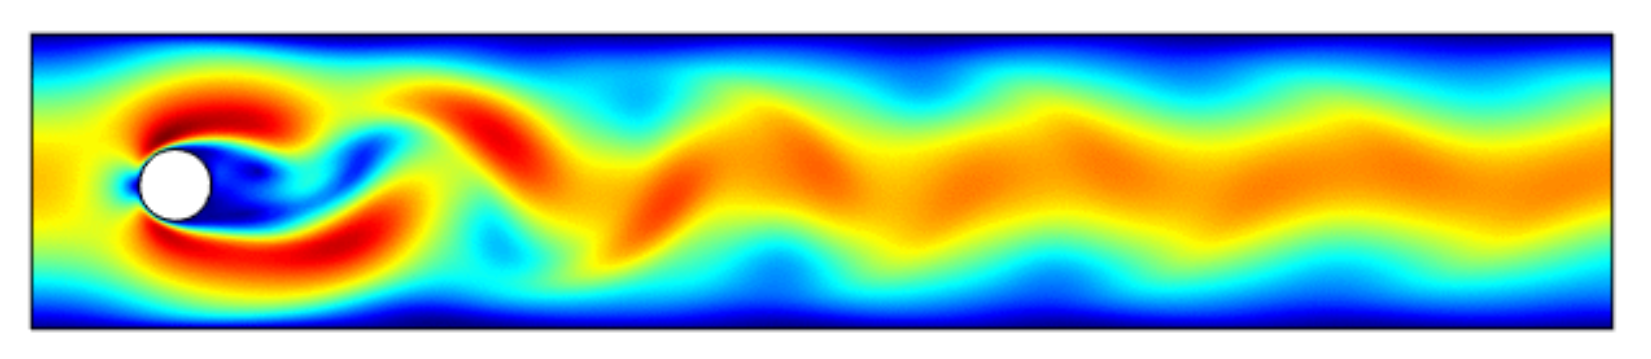
\includegraphics[width=0.9\linewidth]{速度分布.png}}
  \subfigure[压力分布]{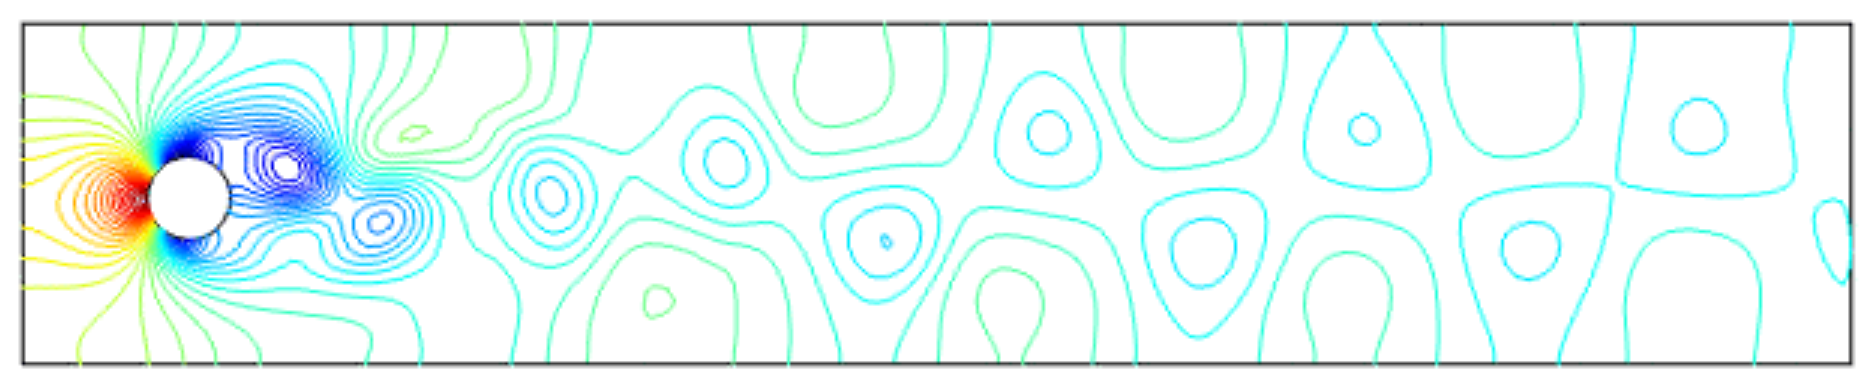
\includegraphics[width=0.9\linewidth]{压力分布.png}}
  \caption{卡门涡街的速度分布和压力分布}
\end{figure}

\subsection{升力系数}
利用COMSOL软件计算绘图功能,在表达式文本框输入升力系数的表达式:\\\texttt{(- reacf(v)\{N\}*2/(spf.rho*U\_mean\textasciicircum2*(2*R)\{m\textasciicircum2\}))[1/m]}

导出得到图如下:
\begin{figure}[h!]
  \centering
  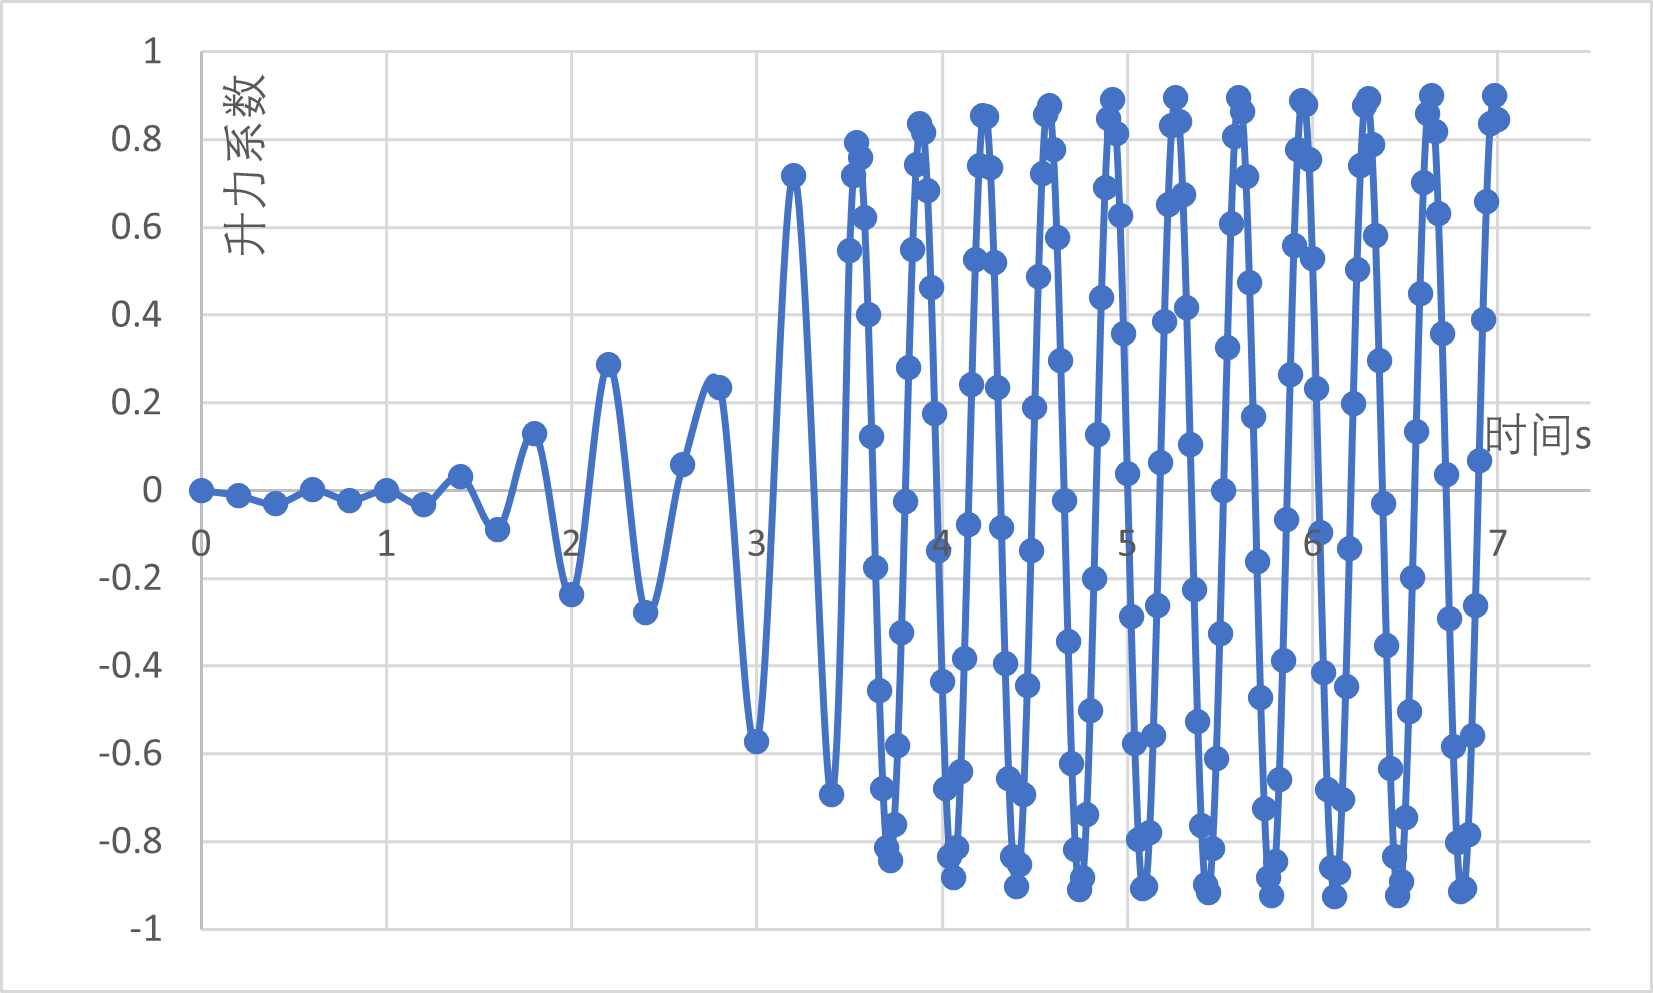
\includegraphics[width=0.7\linewidth]{升力系数.png}
  \caption{升力系数随时间变化图}
\end{figure}

\subsection{曳力系数}
类似步骤,在表达式文本框中输入曳力系数的表达式,选中描述复选框,在关联文本框里输入曳力系数;在一维绘图组4工具栏中单击绘制,看到曳力系数曲线
\begin{figure}[h!]
  \centering
  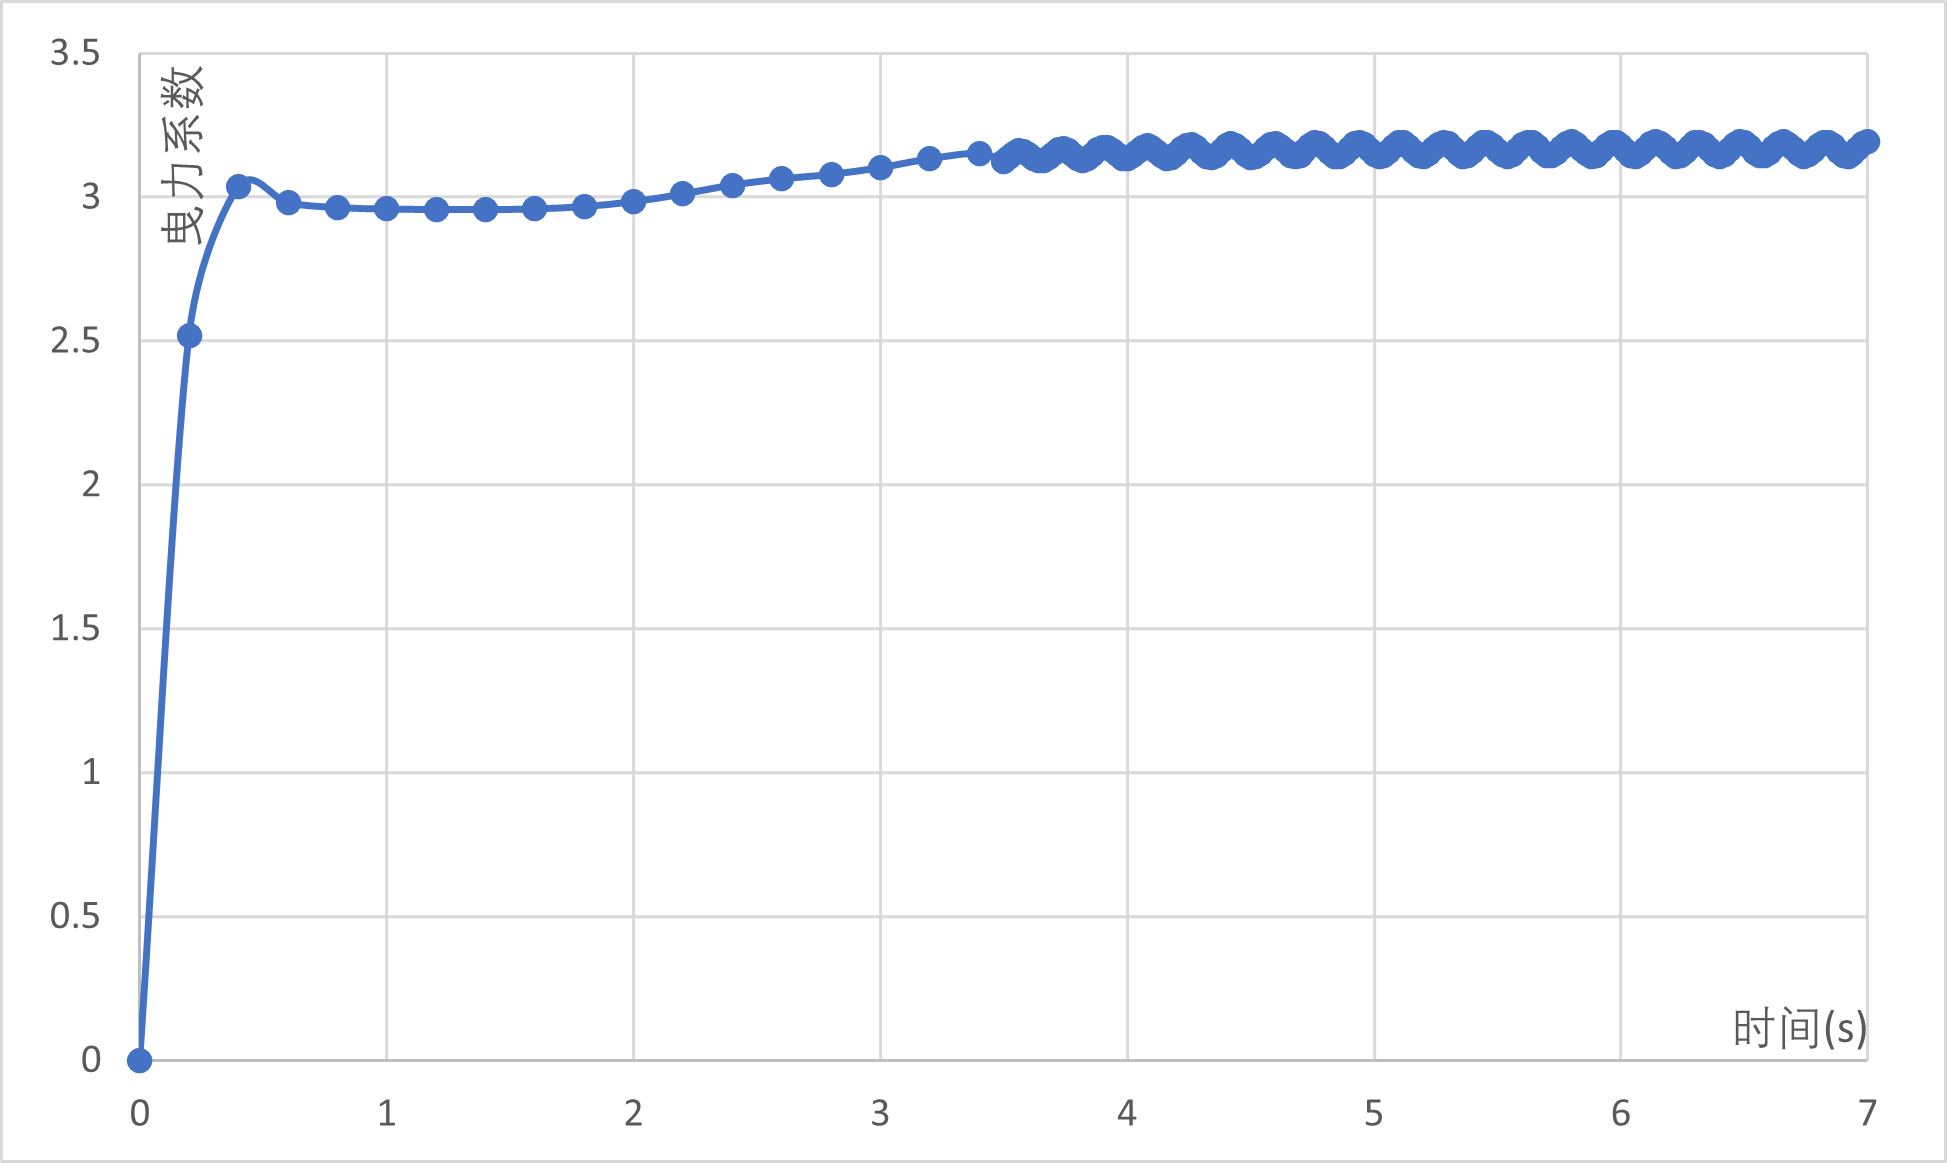
\includegraphics[width=0.7\linewidth]{曳力系数.png}
  \caption{曳力系数随时间变化图}
\end{figure}

\longLine
\section{数据处理}
%(注:需从原始数据记录表整理数据到此栏,再进行数据处理)
\subsection{根据升力系数峰值估算振动频率和升力大小}
1. 选取升力系数6个峰值或谷值(3.5s之后的点);\\
利用公式\ref{eq:CLCD}计算升力大小:
$$F_L=\frac{1}{2}C_L \rho u^2 A$$
例如$F_{L,t=4.92}=\frac{1}{2}\times0.890\times1\times1^2\times1\times0.05\times2\approx\qty{44.52}{mN}$

\begin{table}[h!]
  \centering
  \begin{tabular}{@{}lllllll@{}}
  \toprule
  % t(s)   & 4.92  & 6.30  & 5.60  & 5.26  & 6.64  & 6.98  \\ \midrule
  t(s)   & 4.92  & 5.26 & 5.60 & 6.30  & 6.64 & 6.98 \\
$C_L$     & 0.890 & 0.896 & 0.895 & 0.892 & 0.899 & 0.901 \\
$F_L$(mN) & 44.52 & 44.81 & 44.77 & 44.62 & 44.97 & 45.06 \\ \bottomrule
  \end{tabular}
  \caption{升力系数峰值}
  \end{table}

2. 每两个相邻峰(或谷)之间的时间差近似为一个周期,用逐差
法计算振动的周期;

用逐差法计算振动周期:
$$T=\frac{(t_4+t_5+t_6)-(t_1+t_2+t_3)}{3\times3}=\frac{6.30+6.64+6.98-4.92-5.26-5.60}{3\times3}=\frac{4.14}{9}\approx\qty{0.46}{s}$$

3. 根据周期计算卡门涡街的振动频率;
振动频率约为$f=\frac{1}{T}=\frac{1}{0.46}\approx\qty{2.17}{Hz}$

4. 假设圆柱长度为$\qty{1}{m}$,由升力系数定义,计算升力的峰值。
升力峰值:$$F_L=\frac{F_1+F_2+F_3+F_4+F_5+F_6}{6}=\frac{44.52+44.62+44.77+44.81+44.97+45.06}{6}\approx\qty{44.8}{mN}$$

\subsection{根据曳力系数的稳定值估算曳力大小}
由于曳力逐渐趋于一个稳定值,在稳定值区域选取3.1用来估算曳力大小。

假设金属柱长度为\qty{1}{m},根据曳力系数定义,利用公式\ref{eq:CLCD},曳力大小
$$F_D=\frac{1}{2}C_D \rho u^2 A\approx\frac{1}{2}\times3.1\times1\times1^2\times1\times0.05\times2\approx\qty{155.0}{mN}$$


\longLine
\section{结果陈述}
计算结果显示,经卡门涡街影响,圆柱体在竖直方向的升力峰值约为$\qty{44.8}{mN}$,在水平方向的曳力峰值约为$\qty{155.0}{mN}$,升力峰值约为曳力峰值的$29\%$。圆柱体在竖直方向所受升力远小于水平方向的曳力。然而,竖直方向的升力方向在不断改变,改变的频率约为$\qty{2.17}{Hz}$,而水平方向的曳力方向始终不变,保持与流体方向相反。尽管升力方向受力较小,流体的卡门涡街振动可能对结构产生影响,因此在实际应用中需要避免结构的固有频率与其接近。

\longLine
\section{实验总结与思考题}
\subsection{实验总结}
本次实验通过COMSOL软件的数值模拟,我可以更加直观地了解圆柱体在卡门涡街流场中的受力情况,并且可以通过改变流场参数等方式,这对于我们深入理解卡门涡街现象及其对结构的影响具有重要的意义。

之后,我计算了升力曳力系数,对流体有了初步认识,对流体力学的原理方程有了初步了解。

通过本次实验,我不仅感受了流体力学实验的基本方法和技能,还学习了使用COMSOL软件进行数值模拟的方法,这对于我们今后的学习和研究具有重要的意义,这是一次有趣的实验。
\subsection{思考题}
\subsubsection{为什么升力系数随时间振荡?这在实际中带来哪些影响?请举例说明}
\textbf{答:}升力系数随时间振荡的原因是由于流体在通过圆柱体等物体时,会形成一系列交替脱落的涡旋,这些涡旋会引起物体周围的压力变化。这种压力变化会导致圆柱体所受升力的大小和方向随时间发生变化,从而导致升力系数随时间振荡。

升力系数的大小和方向与伯努利方程有关。伯努利方程(公式\ref{eq:bernoulli})描述了流体在不同位置的压力、速度和高度之间的关系,速度越大,压强越小,而在圆柱体等物体周围,由于流体速度的变化,压力也会发生变化,从而导致圆柱体所受升力的大小和方向发生变化。

在实际中,升力系数随时间振荡可能会对结构产生影响。例如,在飞行器乃至高楼设计中,如果结构的固有频率与流体的卡门涡街频率接近,就可能会导致结构受到共振的影响,从而引起结构的破坏。因此,在设计飞行器等结构时,需要考虑流体的卡门涡街频率,并尽可能避免结构的固有频率与其接近。

\subsubsection{简述卡门涡街流量计的工作原理}
\textbf{答:}卡门涡街流量计是一种测量流体流量的仪器。它的工作原理基于卡门涡街的现象,即在流体通过圆柱体等物体时,会形成一系列交替脱落的涡旋,这些涡旋会引起物体周围的压力变化。卡门涡街流量计利用这种现象,通过测量涡旋脱落的频率来计算流体的流量。

卡门涡街流量计通常由一个圆柱体和一个压电传感器组成。当流体通过圆柱体时,会形成涡旋并引起压力变化,这些压力变化会被传感器检测到并转换为电信号。通过测量涡旋脱落的频率,可以计算出流体的流量。

一般而言,卡门涡街流量计具有结构简单、精度高、可靠性好等优点,广泛应用于工业生产和科学研究中。

\endBox
\end{document}